\documentclass[revision-guide.tex]{subfiles}
%% Current Author: BC
\setcounter{chapter}{6}
\begin{document}
\chapter{Superposition}
\begin{content}
\item phase difference
\item diffraction
\item interference
\item standing waves
\end{content}

\section*{Candidates should be able to:}
\spec{explain and use the concepts of coherence, path difference, superposition and phase}
\spec{understand the origin of phase difference and path difference, and calculate phase differences from path differences}
\spec{understand how the phase of a wave varies with time and position}

These terms are all used when considering more than one wave.

The phase of a wave is related to how far through an oscillation a wave is. This is expressed in radians or degrees, where one complete oscillation corresponds to $360^{\circ}$ or $2\pi$ radians.

The phase difference between two waves is more useful than the phase of one wave. This refers to the fraction of an oscillation by which one wave 'leads' or 'lags' behind another. If the phase difference is $2n\pi$, where $n$ is an integer, then two waves are said to be \emph{in phase} and if the phase difference is $(2n-1)\pi$ then the waves are completely \emph{out of phase}.

Two waves are said to be coherent if they have a constant phase difference. Most often, this is a phase difference of zero, which means that the waves are in phase, but this does not always have to be the case. For interference patterns to occur, coherence is often a necessary condition.

If two waves, from two different sources, meet at a point, the path difference is the difference in distance travelled between the two waves. To calculate the path difference the smaller distance should be taken away from the larger distance. Path difference is normally expressed as a multiple of wavelength, as this then allows the phase difference to be calculated easily.

When two or more waves meet at a point, superposition will occur. This means that the displacements of the individual waves add up to give a resultant displacement. If the two waves are in phase, then constructive interference will occur and if they are out of phase then destructive interference will occur.

\begin{center}
\begin{tabular}{c|c|c}
\textbf{Path difference} & \textbf{Phase difference} & \textbf{Superposition}\\
\hline
$n\lambda$ & $2n\pi$ & constructive interference\\
\hline
$(n+\frac{1}{2})\lambda$ & $(2n-1)\pi$ & destructive interference
\end{tabular}
\end{center}

\spec{determine the resultant amplitude when two waves superpose, making use of phasor diagrams}

When two waves superpose, the resultant displacement at any point is the vector sum of the individual displacements.

\begin{figure}[h!]
\centering
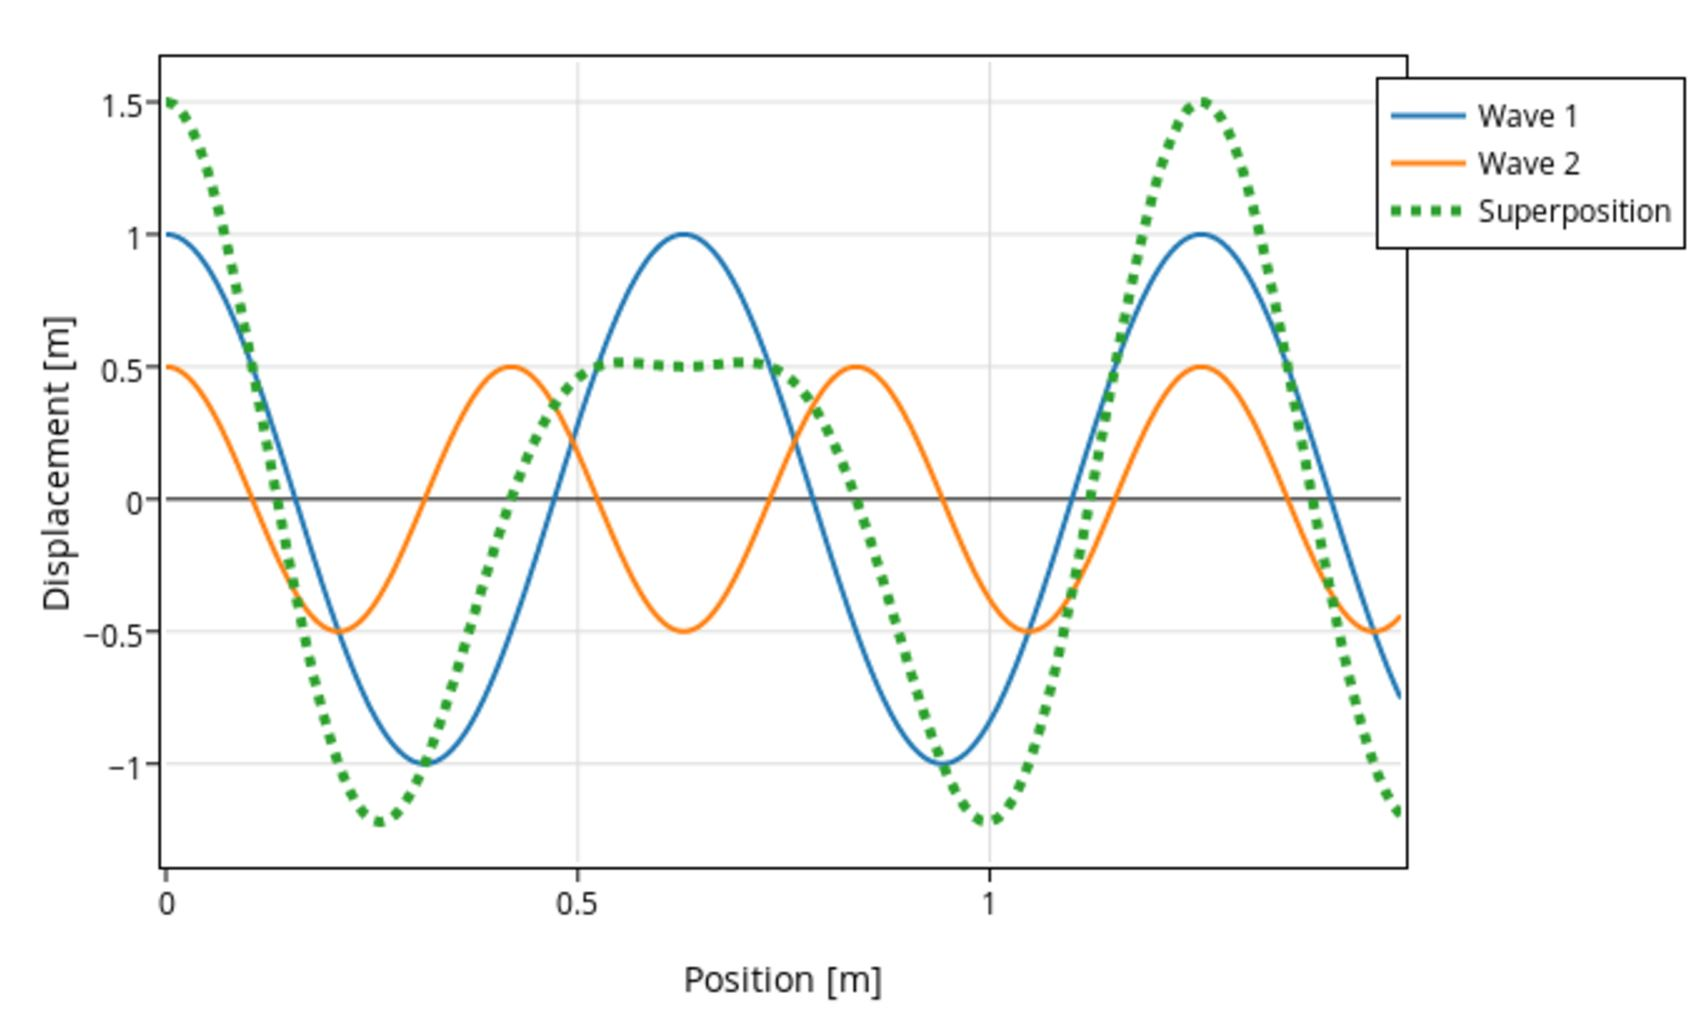
\includegraphics[width=10 cm]{figs/chapt-7/superposition.JPG}
\caption{Graph showing superposition of two waves}
\end{figure}

Phasors are rotating arrows that can be used to describe waves. A phasor arrow rotates anticlockwise and one full oscillation of the wave corresponds to one complete oscillation of the phasor arrow. The length of the phasor arrow corresponds to the amplitude of the wave. 

\begin{figure}[h]
\centering
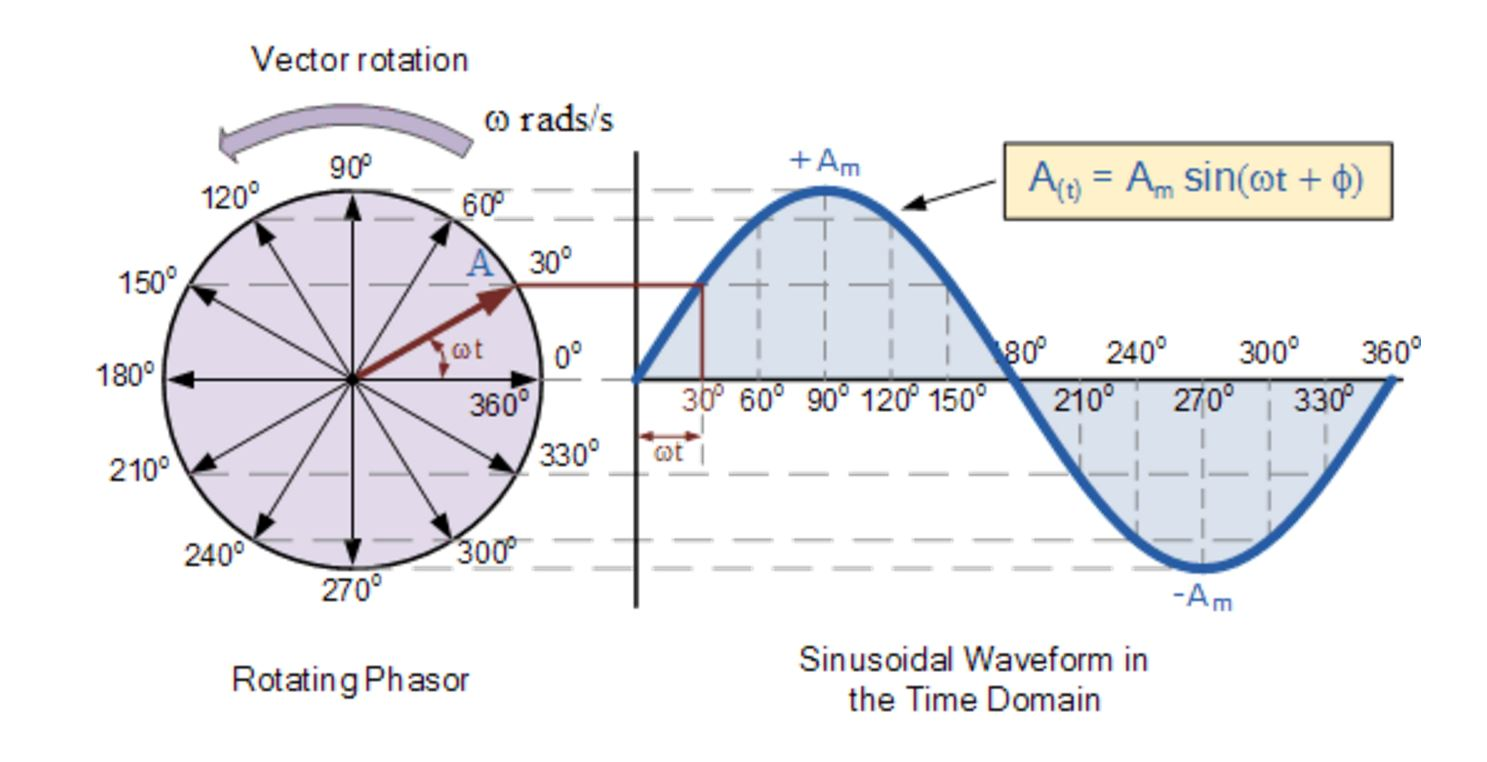
\includegraphics[width=\textwidth]{figs/chapt-7/phasor.JPG}
\caption{The circle on the left shows the rotating phasors that correspond to this sine wave}
\end{figure}

If we have two waves that superpose, their individual phasor arrows at a particular point can be added up as vectors as shown in the diagram below.

\begin{figure}[h]
\centering
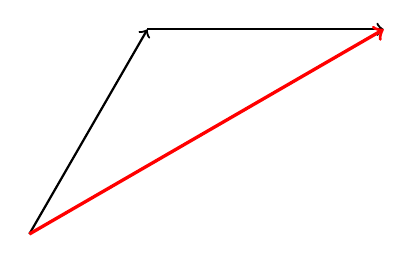
\begin{tikzpicture}
    \draw[thick,->] (0,0) -- (1.5,2.6);
    \draw[thick,->] (1.5,2.6) -- +(3,0);
    \draw[very thick, red,->] (0,0) -- (4.5,2.6);
\end{tikzpicture}
\caption{The sum of two phasors placed end to end}
\end{figure}

\spec{explain what is meant by a standing wave, how such a wave can be formed, and identify nodes and antinodes}

A standing wave arises from a combination of reflection and interference. Consider the set up below.

\begin{figure}[h!]
\centering
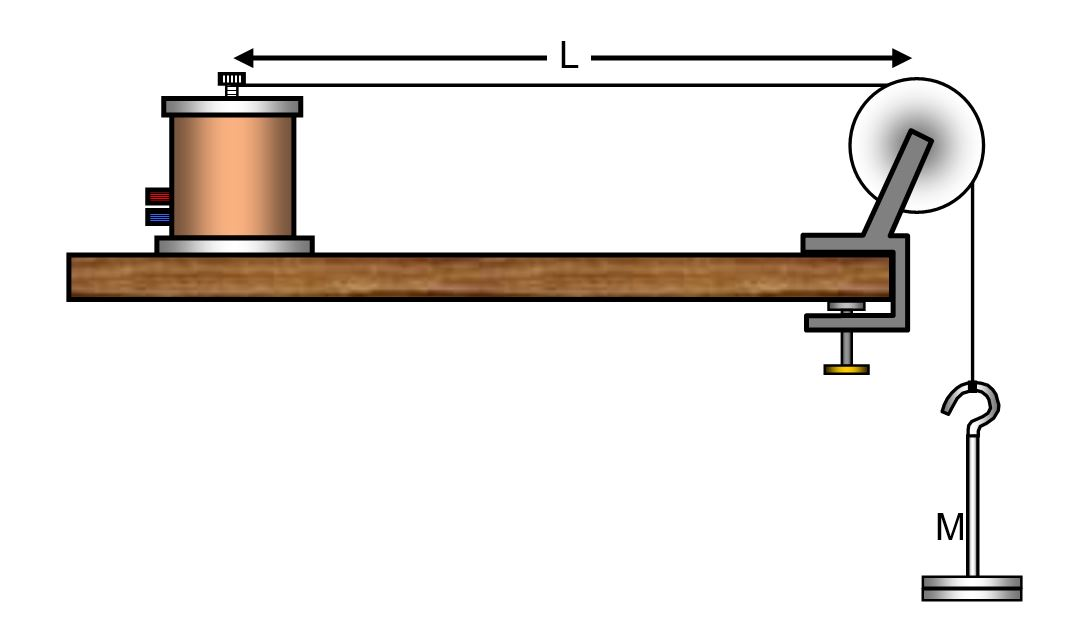
\includegraphics[width=10cm]{figs/chapt-7/melde.JPG}
\caption{Vibration generator connected to a horizontal string under tension}
\end{figure}

The vibration generator leads to a progressive wave travelling to the right. This waves reflects off the fixed end and so there are now two waves on the string, travelling in opposite directions.

These two waves superpose and, in some cases (conditions discussed below), a standing wave can form on the string. If these conditions are met, there will be points where the two waves always meet in phase and interfere constructively. These are called \emph{antinodes}. The points where the two waves always meet out of phase and interfere destructively are called \emph{nodes}.

\begin{figure}[h!]
\centering
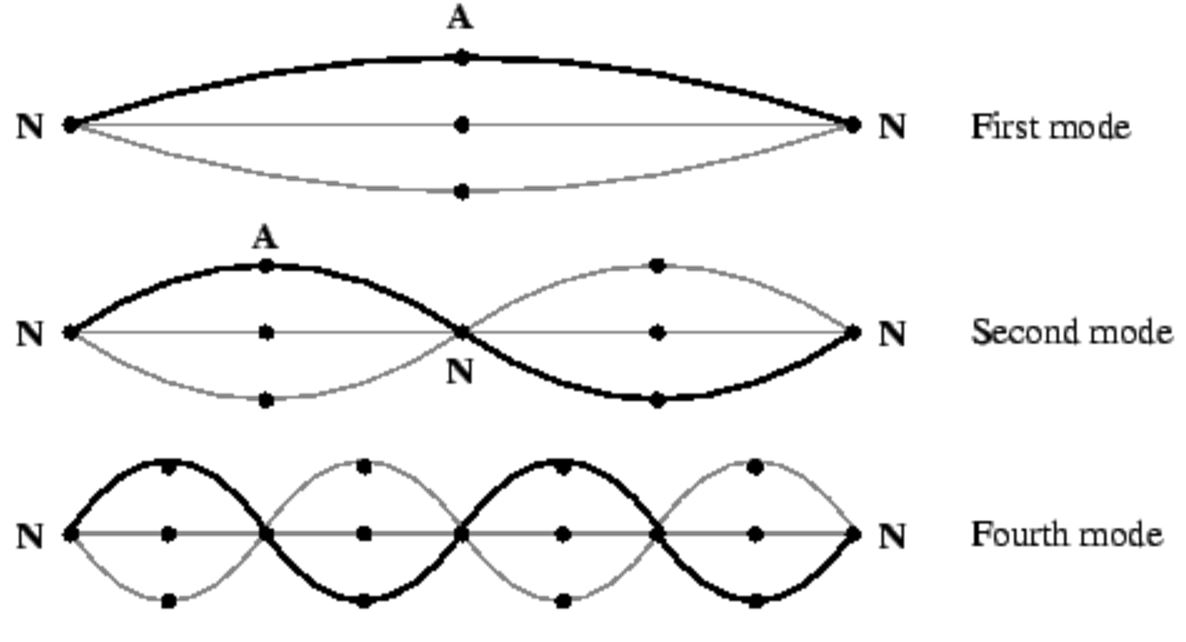
\includegraphics[width=10cm]{figs/chapt-7/string.JPG}
\caption{modes of oscillation on a string}
\end{figure}

Unlike a progressive wave, all points on a stationary wave do not have the same amplitude. The amplitude is at a minimum (often zero) at a node and at a maximum at an antinode.

If the length of the string is $L$, and the speed of waves on the string is $v$, we can work out the frequencies of the various modes of oscillation. The lowest frequency (first mode) shown in the diagram is called the fundamental frequency. You can see that half of a wavelength fits on the string. Therefore we can write:
$$\frac{\lambda}{2} = L$$
$$\lambda = 2L$$

Putting this into the wave equation gives an expression for the fundamental frequency:
$$v = f\lambda = f.2L$$
$$f = \frac{v}{2L}$$

The other modes of oscillation can be worked out in similar ways, by looking at the relationship between $L$ and $\lambda$ and substituting into the wave equation. For a given string under a certain tension the speed is constant. The frequency is the frequency of the vibration generator which can be changed to give the different modes of oscillation.

The boundary conditions for this string were that both ends had to be nodes. In other cases where standing waves occur, for example sound waves, the boundary conditions could be different. Closed ends of tubes are always nodes and open ends are always antinodes.

\begin{figure}[h!]
\centering
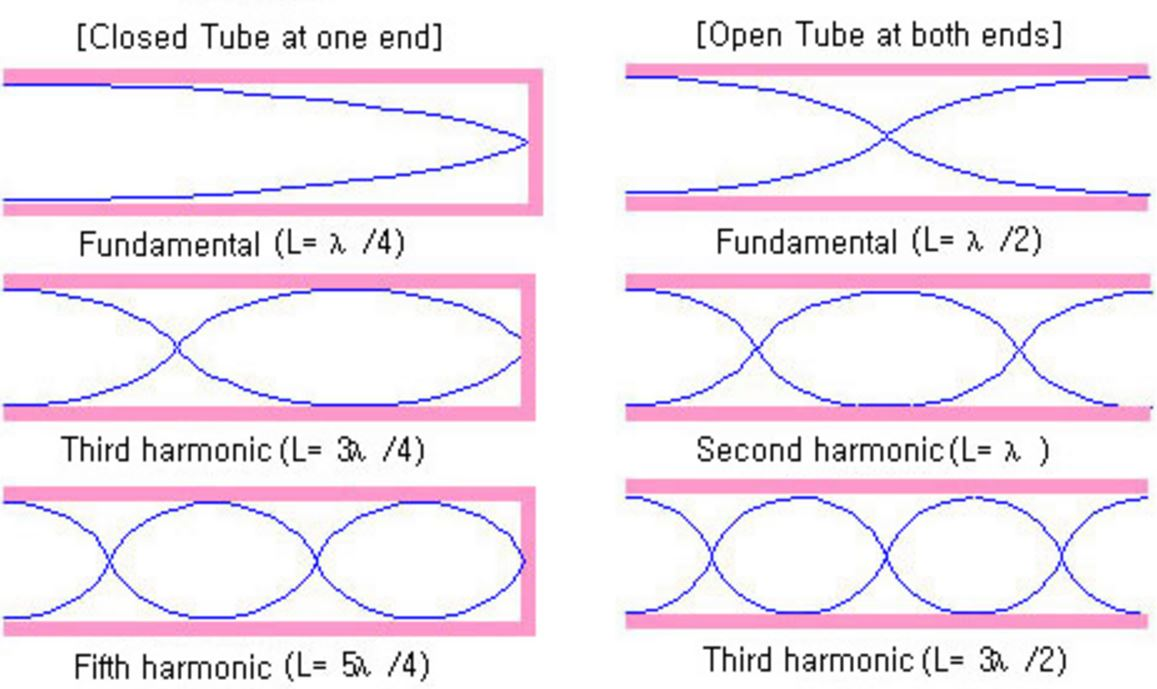
\includegraphics[width=10cm]{figs/chapt-7/sound.JPG}
\caption{Standing waves in a tube {credit:Yonsei Phylab}}
\end{figure}

\spec{understand that a complex wave may be regarded as a superposition of sinusoidal waves of appropriate amplitudes, frequencies and phases}

If more than two waves superpose, the resultant wave can get very complicated! This means that \emph{any} waveform can always be broken down into sinusoidal waves. With combinations of sinusoidal waves of various frequencies, amplitudes and phase differences, any waveform can be made.

\begin{figure}[h!]
\centering
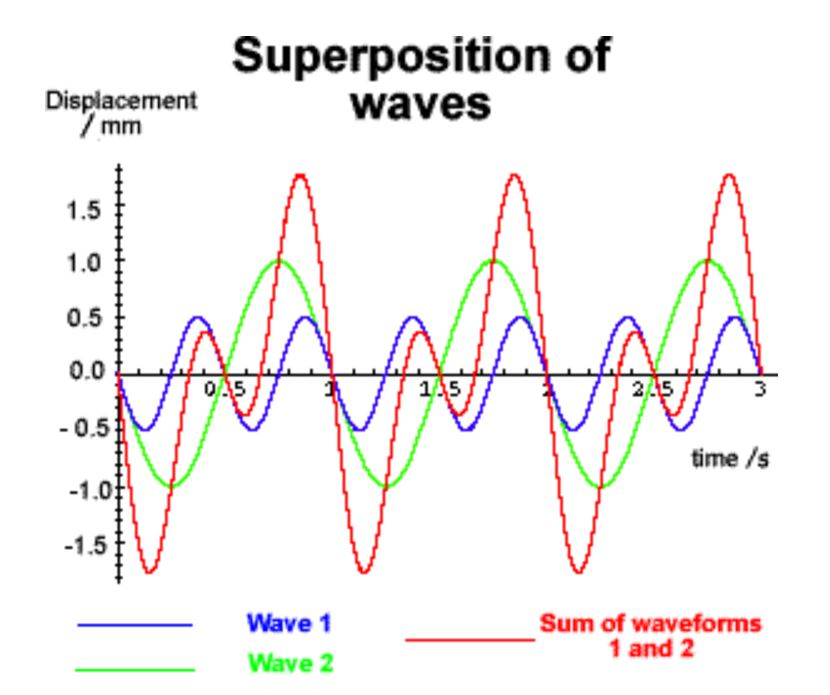
\includegraphics[width=10cm]{figs/chapt-7/sine1.JPG}
\caption Example showing how 2 waves combine to form a more complex wave (credit:cyberphysics.co.uk)
\end{figure}

\spec{recall that waves can be diffracted and that substantial diffraction occurs when the size of the gap or obstacle is comparable to the wavelength}

\spec{recall qualitatively the diffraction patterns for a slit, a circular hole and a straight edge}

When waves pass through an opening, or around a barrier, diffraction occurs and the waves can change in direction and spread out. Diffraction is most significant when the size of the gap or obstacle is comparable to the wavelength. For example, sound waves will diffract through open doors as they have wavelengths of similar orders of magnitudes to the size of the door. However, light will not diffract as much through a door as the wavelength of light is many orders of magnitude smaller than the size of the door.

When waves diffract, diffraction patterns will be formed due to interference of the waves. Specific cases will be discussed below. Here are some examples of diffraction patterns:

\textbf{A slit}

When a wave passes through a slit, and the wave is observed a certain distance away from the slit, a diffraction pattern consisting of points of constructive interference and destructive interference will be formed. Visible patterns will occur when the size of the slit is comparable to the wavelength. For example, with visible light and a very narrow slit, the following pattern will be observed.

\begin{figure}[h!]
\centering
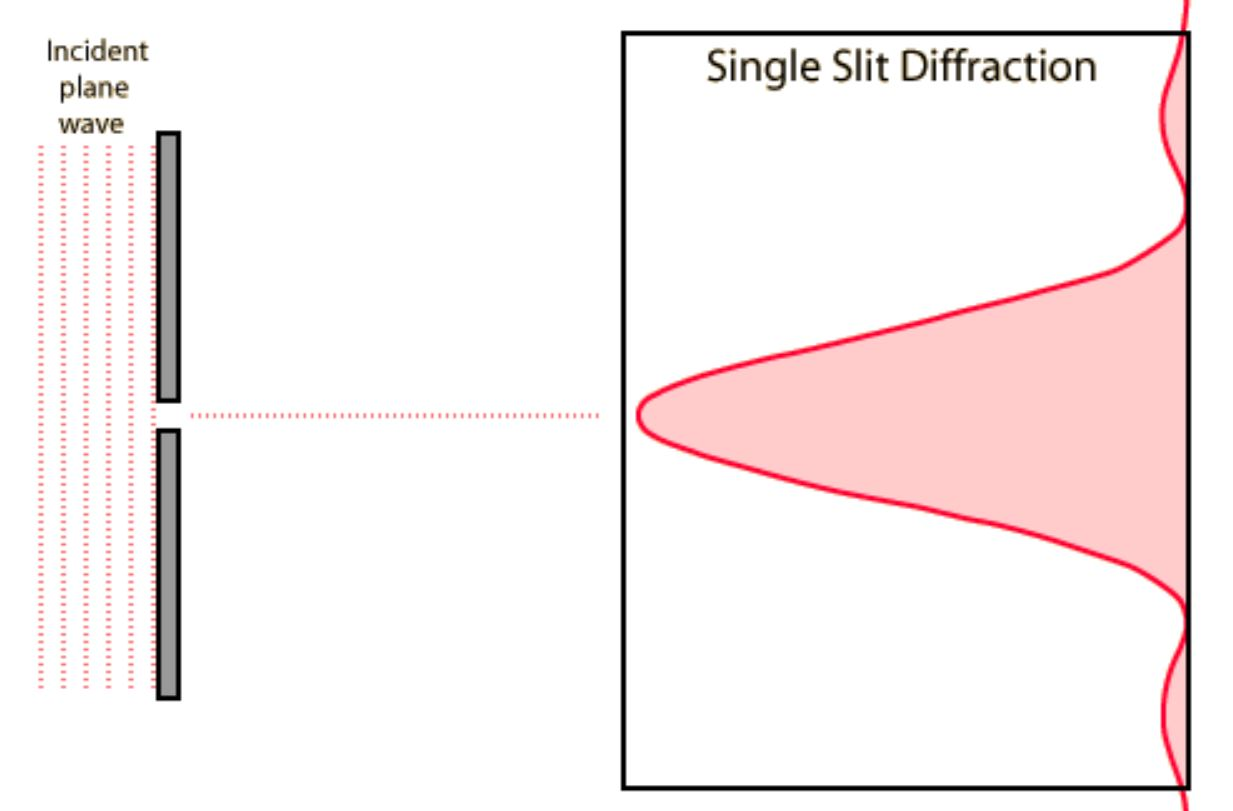
\includegraphics[width=10cm]{figs/chapt-7/slit.JPG}
\caption{Diffraction pattern for a slit (credit:hyperphysics)}
\end{figure}

There is a central maximum which is twice the width of the maxima on either side and the pattern is symmetrical.

\begin{figure}[h!]
\centering
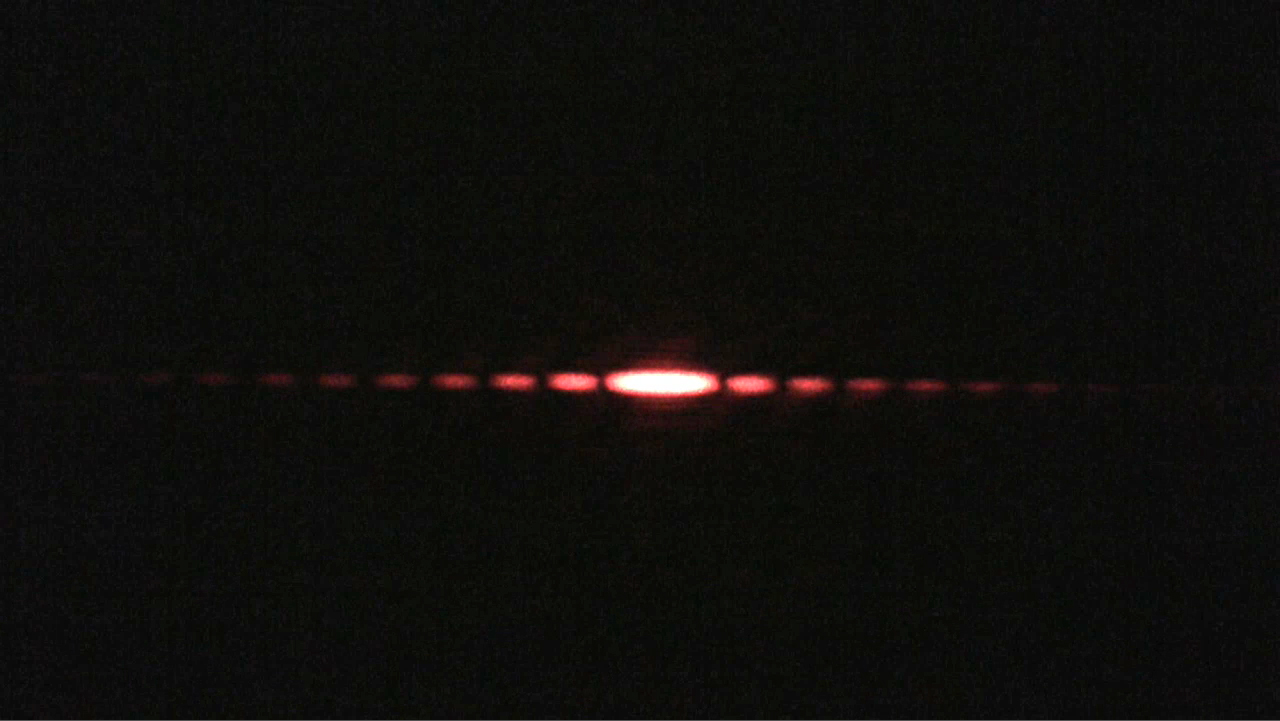
\includegraphics[width=10cm]{figs/chapt-7/slitphoto.jpg}
\caption{Photograph of single slit diffraction pattern}
\end{figure}

\textbf{A circular hole}

The diffraction pattern for a circular hole is similar to a single slit, except that instead of fringes, the pattern consists of rings.

\begin{figure}[h!]
\centering
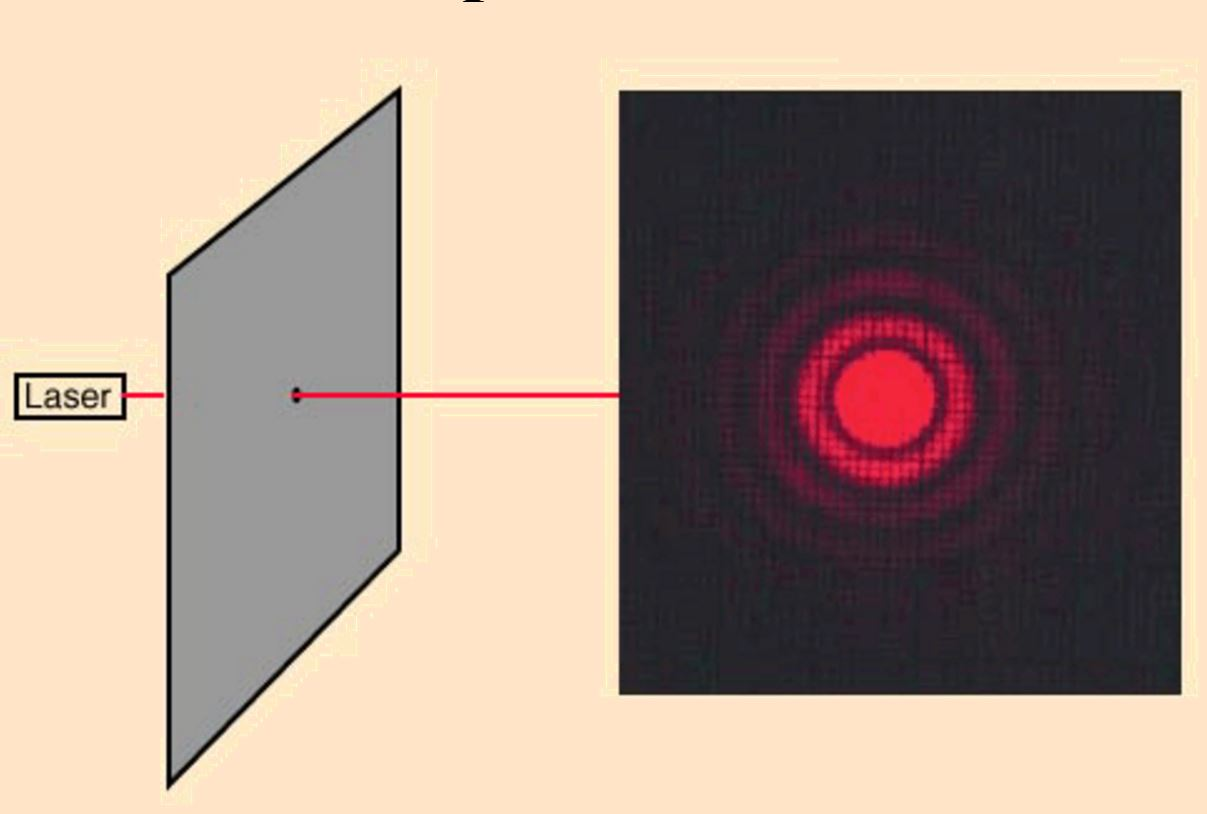
\includegraphics[width=10cm]{figs/chapt-7/hole.JPG}
\caption{Circular hole diffraction pattern {credit:hyperphysics}}
\end{figure}

Although the examples given here are for visible light, remember that \emph{all} waves can diffract.

\textbf{A straight edge}

A similar pattern of fringes is seen, due to constructive and destructive interference. Here the example given is for radio waves.

\begin{figure}[h!]
\centering
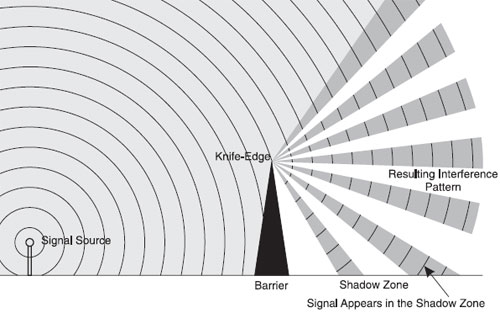
\includegraphics[width=10cm]{figs/chapt-7/edge.jpg}
\caption{Diffraction at a straight edge {credit:University of Alberta}}
\end{figure}

\spec{recognise and use the equation $n\lambda = b sin\theta$ to locate the positions of destructive superposition for single slit diffraction, where $b$ is the width of the slit}

When an electromagnetic wave, such as light, travels through a single slit, it will diffract. Therefore light from the slit reaches many points on a screen placed at some distance from the slit.

Consider a point on the screen. Light will reach this point from all points within the slit. The distances travelled from various points within the slit to the point on the screen will be different, and so there will be a path and phase difference. Therefore, as we move along the screen, there will be points of constructive interference and points of destructive interference.

\begin{figure}[h!]
\centering
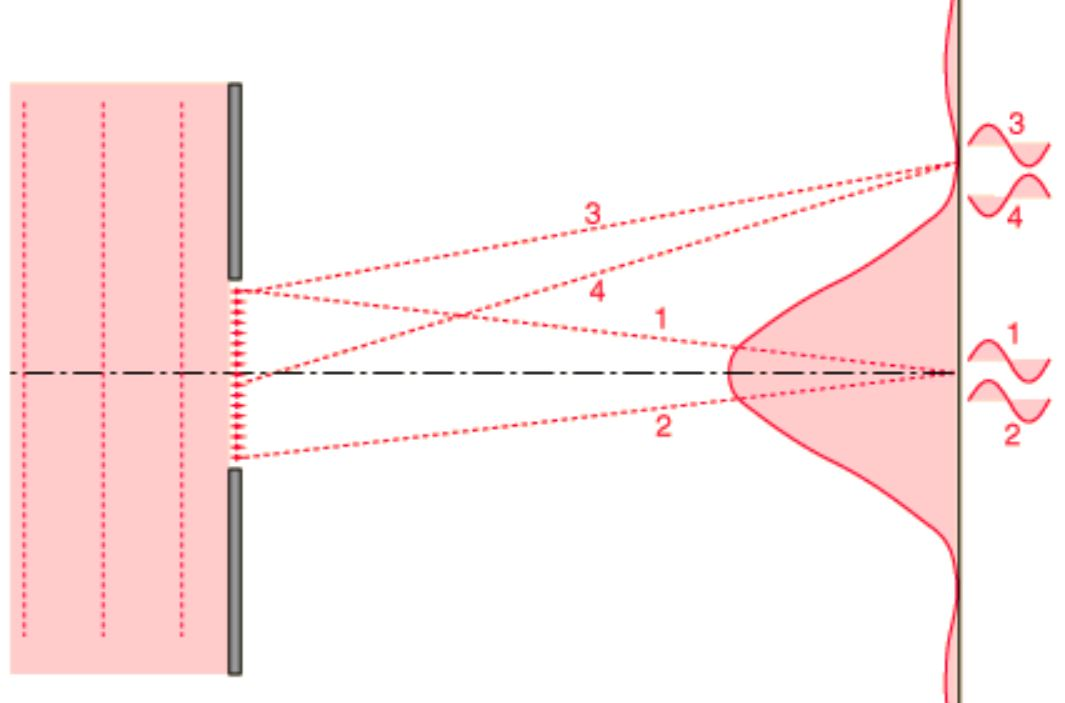
\includegraphics[width=10cm]{figs/chapt-7/singleslit.JPG}
\caption{Single slit diffraction {credit:hyperphysics}}
\end{figure}

It can be shown that for a single slit of width $b$, the points of \textbf{destructive interference} will be at an angle $\theta$ given by the equation
$n\lambda = b sin\theta$
Here, $n$, refers to the order of the minimum being considered.

\spec{recognise and use the Rayleigh criterion $\theta \approx \frac{\lambda}{b}$ for resolving power of a single aperture, where $b$ is the width of the aperture}

As light travels through an instrument, such as the eye, or a telescope, it passes through a gap or aperture and will diffract. The diffraction pattern will depend on the shape of the aperture and the width.

If light from two different objects passes through the aperture, there will be two diffraction patterns that overlap. The Rayleigh criterion tells us the minimum angle between the two objects at which it is still possible to see them as separate. This is when the first diffraction minimum of one pattern coincides with the central maximum of another.

Working in radians, so that the approximation $\sin{\theta} \approx \theta$, then this minimum angle can be approximated by:

$$\theta \approx \frac{\lambda}{b}$$

\spec{describe the superposition pattern for a diffraction grating and for a double slit and use the equation $d \sin\theta = n\lambda$ to calculate the angles of the principal maxima}

\spec{use the equation $\lambda = \frac{ax}{D}$ for double-slit interference using light}

When light, or any other coherent waves, pass through a double slit, a diffraction pattern consisting of evenly spaced fringes is seen. This is due to the waves from each slit interfering with each other.

\begin{figure}[h!]
\centering
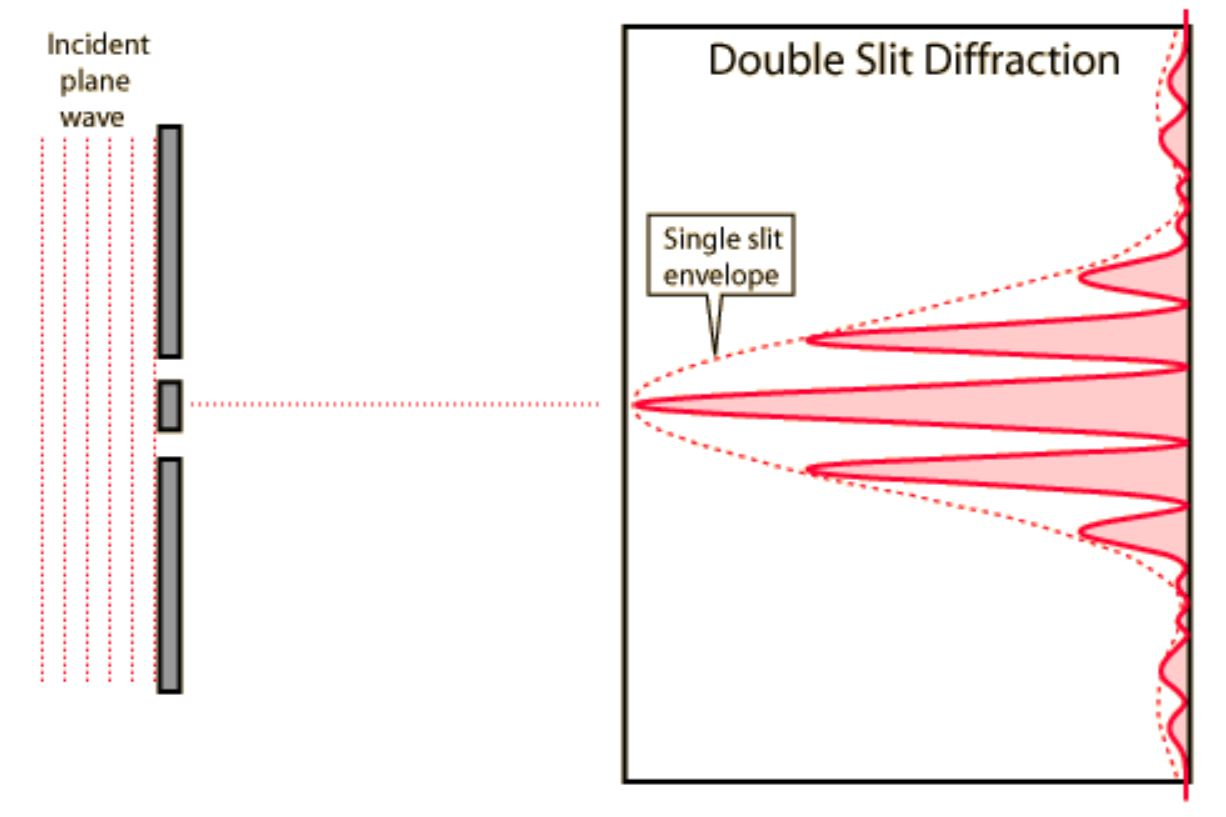
\includegraphics[width=10cm]{figs/chapt-7/double.JPG}
\caption{Double slit diffraction (credit:hyperphysics)}
\end{figure}

You can see that there is also a single slit envelope, which is much wider than the double slit pattern.

If the number of slits is increased, the pattern becomes more defined, and the fringes get narrower. Therefore for a diffraction grating, the pattern consists of sharp, evenly spaced peaks or bright spots.

If we consider two adjacent slits, you can see that for constructive interference to occur the following must be true:

\begin{equation}\label{dsintheta}
d \sin\theta = n\lambda
\end{equation}

$d$ is the distance between adjacent slits and $n$ is the order of the maxima that is being considered.

\begin{figure}[h!]
\centering
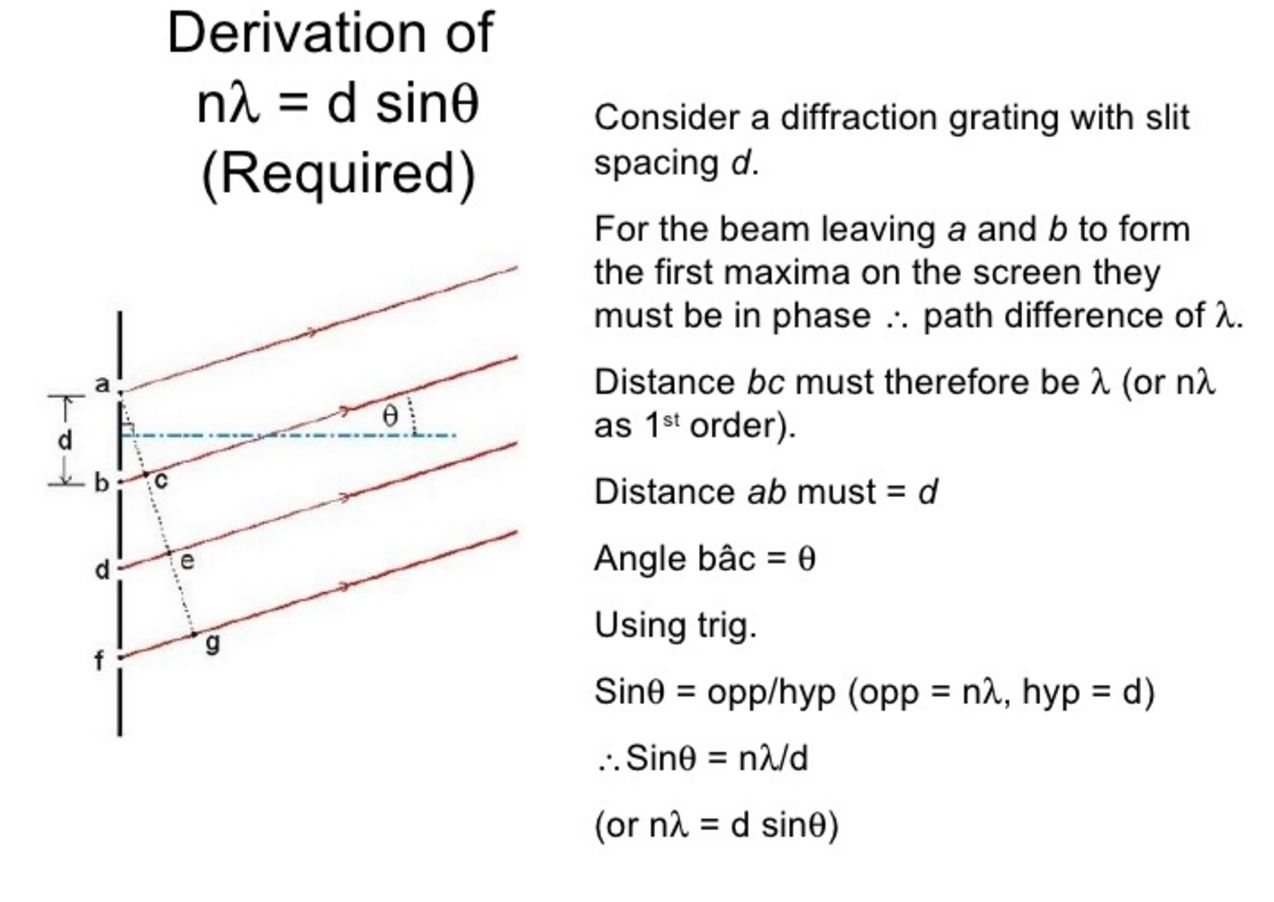
\includegraphics[width=10cm]{figs/chapt-7/diffractioneq.JPG}
\caption{Derivation of grating formula}
\end{figure}

Equation \ref{dsintheta} can be re-arranged to give

\begin{equation}
\sin\theta = \frac{n\lambda}{d}
\end{equation}

This formula can be used for any waves, where there is diffraction from more than one slit.

\newpage

\begin{figure}[h]
    \centering
    \begin{tikzpicture}
    \draw[very thick] (0,-.5) -- (0,.5);
    \draw[thick] (7,-3) -- (7,3);
    \draw[<->] (0,-1) -- (7,-1) node[midway, below] {$D$};
    \draw[dashed] (0,0)--(7,0);
    \draw[red,thick,->] (0,0) -- (7,2);
    \draw[<->] (7.5,0)--(7.5,2) node[midway, right] {$x$};
    \end{tikzpicture}
    \caption{The double slit pattern}
    \label{doubleslitscreen}
\end{figure}

Now consider a double slit pattern, where the screen is now a distance $D$ away from the slits and the slit separation is $a$ instead of $d$. Bright fringes will be equally spaced on the screen and we can call the fringe separation $x$.



For the first maxima, $n=1$, the equation from before now becomes:
$$\sin\theta = \frac{\lambda}{a}$$
but from the diagram you can see that:
$$\tan\theta = \frac{x}{D}$$

If $\theta$ is small, then the small angle approximation can be used. This is true if $D$ is much larger than $a$.

$$\sin\theta \approx \tan\theta$$
$$\frac{\lambda}{a} = \frac{x}{D}$$
$$\lambda = \frac{ax}{D}$$

\end{document}
